%!tex program = lualatex
\documentclass{exam}
\usepackage{ctex}
\usepackage{graphicx}
\usepackage[margin=2cm]{geometry}
\usepackage{amsmath, amssymb}
\usepackage{csquotes}
\usepackage{tikz, pgfplots}
\usetikzlibrary{
	angles,
	backgrounds,
	calc,
	decorations.pathmorphing,
	decorations.pathreplacing,
	decorations.text,
	intersections,
	patterns,
	quotes,
	shapes,
	shapes.symbols,
}
\pagestyle{empty}
\newcounter{xcord}
\newcounter{ycord}
\newcounter{total}
\renewcommand{\labelenumi}{\textbf{\ifnum\value{enumi}<10 0\fi\arabic{enumi})}}

\pgfplotsset{compat=1.18}

\CorrectChoiceEmphasis{\color{blue!70!green}\bfseries}
\renewcommand{\solutiontitle}{\textbf{解:}}

\usepackage{array, tabularx}
\newcolumntype{C}{>{\centering\arraybackslash}X}
\newcolumntype{B}{>{\centering\bfseries\arraybackslash}X}
\catcode`\幺=0

\begin{document}
\section{求阴影面积}
\begin{figure}[htbp]
	\centering
	\begin{gather*}
		长方形ABCD\\
		AB = 9 \\
		BC = 6 \\
		求阴影面积
	\end{gather*}
	\begin{tikzpicture}[scale=.5]
		\coordinate (A) at (9,0);
		\coordinate (B) at (0,0);
		\coordinate (C) at (0,-6);
		\coordinate (D) at (9, -6);
		\coordinate (E) at (3, 0);
		\coordinate (F) at (5, -6);
		\coordinate (C') at (9, -3);
		\coordinate (B') at ($(C') ! 1.2 ! -90:(F)$);
		\path [name path=B'C'] (B') -- (C');
		\path [name path=AE] (A) -- (E);

		\draw [name intersections={of=B'C' and AE, by=G}];
		\node [above right] at(G){$G$};

		% \path[draw=red] {AE};

		\draw[dashed](B) -- (E);
		\draw (E)-- (A) -- (D) -- (F) -- (E);
		\draw[dashed] (F) -- (C) -- (B);
		\draw (F) -- (C') -- (B') -- (E);

		\draw [pattern=north east lines](E) -- (G) -- (C') -- (F) -- cycle;
		\node at (A)[above right]{$A$};
		\node at (B)[above left]{$B$};
		\node at (C)[below left]{$C$};
		\node at (D)[below right]{$D$};
		\node at (F)[below]{$F$};
		\node at (C')[right]{$C\prime$ 中点};
		\node at (E)[above left]{$E$};
		\node at (B')[right, xshift=5pt]{$B\prime$};
	\end{tikzpicture}
\end{figure}

\begin{align}
	FC + FD                    & = 9                      \\
	FC^2                       & = FD^2 + DC^2 = FD^2 + 9 \\
	(FC + FD) \times (FC - FD) & = 9                      \\
	FC - FD                    & = 1                      \\
	FC                         & = 5
\end{align}

Calculate the length of $BE$:
\begin{align}
	\triangle CDF            & \approx \triangle CAG                               \\
	\frac{GA}{AC}            & = \frac{CD}{FD} = \frac{3}{4}                       \\
	GA                       & = \frac{9}{4}                                       \\
	GC                       & = \sqrt{GA^2 + AC^2} = \frac{15}{4}                 \\
	BG                       & = BC - GC = 6 - \frac{15}{4}     = \frac{9}{4} = GA \\
	\because \triangle GBE   & \approx \triangle GAC                               \\
	\therefore \triangle GBE & \cong \triangle GAC                                 \\
	BE                       & = AC = 3
\end{align}

\section*{20以内两位数乘法练习}
\begin{center}
	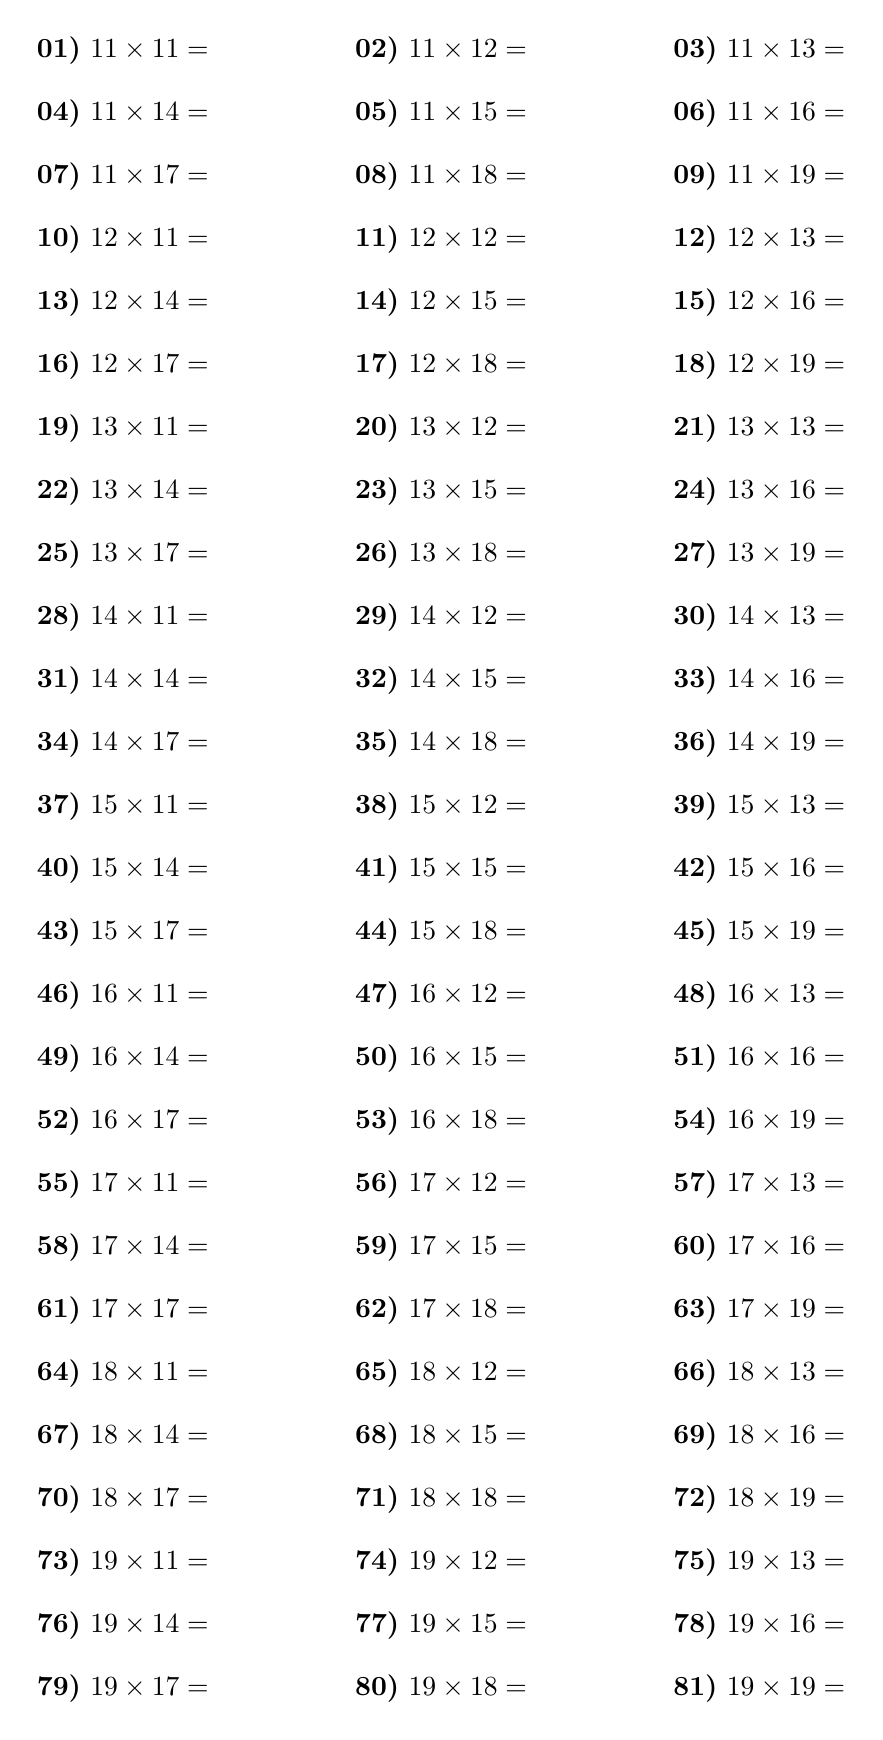
\begin{tikzpicture}
		\foreach \x in {11,...,19}
		\foreach \y in {11,...,19}
			{
				\stepcounter{total}
				\node at (\value{xcord} * \textwidth / 3, -\value{ycord}*0.8) {\textbf{\ifnum\value{total}<10
				0\fi\thetotal)} $\x \times \y =$};
		\stepcounter{xcord}		\ifnum\value{xcord}=3
		\setcounter{xcord}{0}
		\stepcounter{ycord}
		\fi
		}
	\end{tikzpicture}

\end{center}

\section{速算及巧算}
\subsection{计算总和}
\begin{enumerate}[label={\arabic*)}]
	\item \( 1-2+3-4+5-6+7-8+9-10+11=\)
	\item \( 3+5+7+9+11+13+15+17+19+21=\)
	\item \( 100-99+98-97+96-95+94-93+93-92+91=\)
	\item \( 6+8+10+12+14+16+18+20+22+24=\)
	\item \( 1 + 2 + 3 + \ldots + 100 = \)
	\item \( 2 + 4 +6 + \ldots + 100 = \)
	\item \( 1 + 3 + 5 + \ldots + 99 = \)
	\item \( 5 + 10 + 15 + \ldots + 100 = \)
	\item \( 1 - (1+2) + (1+2+3) - (1+2+3+4) + \ldots - (1+2+\ldots+98) + (1+2+\ldots+99) = \)
	\item \( 1-2+3-4+\ldots+2023-2024+2025=\)
	\item \( 19+28+37+46+55+64+73+82+91+ \underline{\hspace{1cm}}=550\)
	\item \( 2000-180+220-180+220-180+220-180+220-180+220=\)
	\item \( 352.46-35.58-65.93-76.07-24.42=\)
	\item \( 1+2+4+8+16+32+64+128+256+512+1024=\)
	\item \( 8+89+899+8999+89999=\)
	\item \( 8+88+888+8888+88888=\)
	\item \( 28+208+2008+20008=\)
	\item \( 24+63+52+17+49+81+74+38+95=\)
	\item \( 1999.9+199.9+19.9+1.9=\)
	\item \( (7+9+11+13+\ldots+37)-(9+11+13+15+\ldots+35)=\)
\end{enumerate}

\pagebreak
\section{速算和巧算2}

\begin{enumerate}[label={\arabic*)}]
	\item \((6+8+10+12+\ldots+36)-(8+10+12+14+\ldots+34)=\)
	\item \((1+4+7+10+\ldots+40)-(4+7+10+13+\ldots+37)=\)
\end{enumerate}
\vskip1cm

一个数除以24得到的结果比这个数除以36得到的结果多9,求这个数是多少?


\begin{enumerate}[label={\arabic*)}]
	\item 首先, 除数越小,得到的商越大,比如 \( 9 \div 3 = 3 \),但是 \( 9 \div 1 = 9 \)
	\item 一个数除以24,意思是将一个大的数平分,每份都是24 
	\item 题目的意思是每份分24时的份数比每份36时的份数要多9份,如下面的图所示
	\item 下图中,左边的部分有多少份我们现在不知道,但是可以知道每一份中,36比24要多12,就是第二行中的蓝色的部分
	\item 第一行中数字全部加起来等于第二行的数字(因为被除数是同一个数)
	\item 所以,第一行中的蓝色部分 \( 24 \times 9 = 216 \)
		应该与第二行中的蓝色部分相等,而第二行中蓝色部分每份是12,所以得到 \( 216 \div 12 = 18 \)份
	\item 那么被除数就应该是 \( 18 \times 36 = 648 \)
	\item 我们还可以反过来验算一下, \( 648 \div 24 = 27 \), \( 648 \div 36 = 18 \), \( 27 - 18 = 9
		\),与题目中给出的条件是一样的。
\end{enumerate}
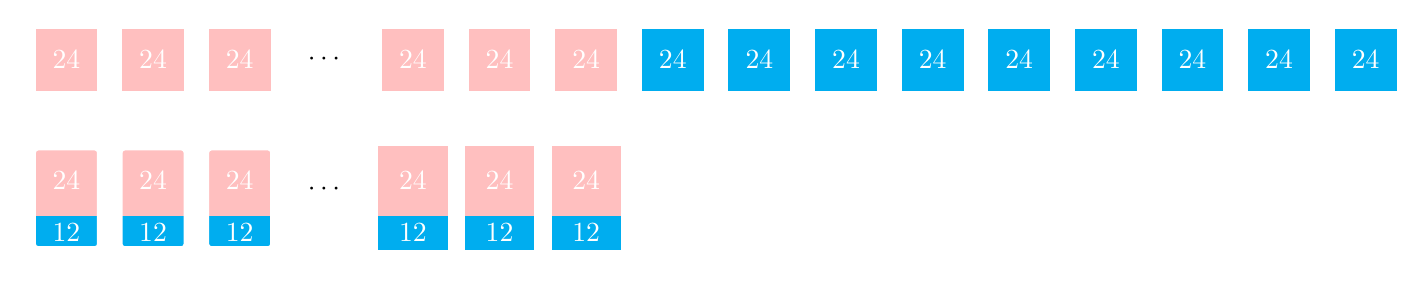
\begin{tikzpicture}[every node/.style={color=white}, scale=1.1]

	% 第一排
	% 粉色矩形(数量未知,使用省略号表示)
	\foreach \i in {1,2,3} {
			\node[draw, fill=pink, minimum width=0.8cm, minimum height=0.8cm] at (\i, 0) {24};
		}
	\node[color=black] at (4, 0) {$\cdots$};
	\foreach \i in {5,...,7} {
			\node[draw, fill=pink, minimum width=0.8cm, minimum height=0.8cm] at (\i, 0) {24};
		}
	% 天蓝色矩形(数量为9)
	\foreach \i in {8,...,16} {
			\node[draw, fill=cyan, minimum width=0.8cm, minimum height=0.8cm] at (\i, 0) {24};
		}

	% 第二排
	% 粉色和天蓝色矩形(分成上下两部分)
	\foreach \i in {1,2,3} {
			\fill[pink] (\i-0.4, -1.8) rectangle  node{24}(\i+0.4, -1);
			\fill[cyan] (\i-0.4, -2.2) rectangle node{12}(\i+0.4, -1.8);
			\draw[rounded corners=2pt, color=white, line width=3pt] (\i-0.4, -2.2) rectangle (\i+0.4, -1);
			% \node at (\i, -1.5) {36};
		}
	\node[black] at (4, -1.5) {$\cdots$};
	\foreach \i in {5,...,7} {
		\draw[white] (\i-0.4, -2) rectangle (\i+0.4, -1);
		\fill[pink] (\i-0.4, -1.8) rectangle node{24} (\i+0.4, -1);
		\fill[cyan] (\i-0.4, -2.2) rectangle  node{12}(\i+0.4, -1.8);
			% \node at (\i, -1.5) {36};
		}

\end{tikzpicture}

\end{document}
